%--------------------------------------------------------------------------
%--------------------------------------------------------------------------
%--------------------------------------------------------------------------
\chapter{Méthode d'Euler}
%--------------------------------------------------------------------------
%--------------------------------------------------------------------------
%--------------------------------------------------------------------------
\section{Équation différentielle}
%--------------------------------------------------------------------------
%--------------------------------------------------------------------------
\subsection{Définitions}
%--------------------------------------------------------------------------

Une équation différentielle (ordinaire) du premier ordre est une équations de la forme
\[ 
y'=\varphi(y,t)\leqno(E)
\]
où $\psi$ est définie sur un ouvert $\cal O$ de $\R^n\times\R$ vers $\R^n$.

Une solution de $(E)$ est une fonction $f$ de classe $\mathcal{C}^1$ sur un intervalle $I$ de $\R$ vers $\R^n$ telle que 

$\bigl(f(t),t\bigr)\in {\cal O}$ et $f'(t)=\psi\bigl(f(t),t\bigr)$ pour tout $t\in I$.

\def\k{-0.25}
\begin{center}
\tikzpicture [scale=0.8] 
\draw[-stealth] (-6,0)--(6,0) node [below] {$t$}; 
\draw[-latex] (0,0)--(1,0); 
\draw[-stealth] (0,-3)--(0,3) node [left] {$y$}; 
\draw[-latex] (0,0)--(0,1); 
\foreach \a in {-5.5,-5,...,5.5}
 \foreach \b in {-2.5,-2,...,2.5}
 \draw[->] (\a,\b)--+(0.2,{0.2*(((3*\a*\a+1)*\k-2*\a*\b)/(\a*\a+1)});
\foreach \c in {-2,0,1,3}
 \draw [samples=100,domain=-5.5:5.5] plot(\x,{\c/(\x*\x+1)+\x*\k});
\endtikzpicture 
\end{center}

Soit $(t_0,y_0)\in U$. Sous certaines conditions sur $\varphi$, le théorème de Cauchy-Lipschitz affirme l'existence et l'unicité d'une solution $(I,f)$ telle que $t_0\in I$ et $f(t_0)=y_0$.

\medskip

On peut alors écrire $\displaystyle f(t) = f(t_0)+\int_{t_0}^t f'(u) \d u
= y_0+\int_t^{t_0} \varphi\bigl(f(u),u\bigr) \d u$.

On a remplacé l'équation différentielle par une équation intégrale.
%--------------------------------------------------------------------------
\subsection{Recherche d'approximation}
%--------------------------------------------------------------------------
Résoudre (on dit aussi intégrer) l'équation différentielle signifie trouver l'unique fonction solution de l'équation pour des conditions initiales données. On cherchera une solution {\bf sur} un segment déterminé, on admettra qu'il existe une solution sur cet intervalle. 

Le temps initial doit appartenir au segment : on simplifiera l'étude en supposant que l'intervalle d'étude commence en $t_0=a$ : $[a;b]$. Les algorithmes proposés seront utilisables aussi si on a $b < a$.
Si la condition initiale était donnée au temps $t_0 \in ]a;b[$ on diviserait l'étude sur deux intervalles : $[a;t_0]$ et $[t_0;b]$.

Une solution est une fonction, on souhaite la valeur en tout temps $t$ de l'intervalle. Malheureusement il est illusoire d'espérer calculer une "formule" de la solution. On se contente donc de calculer la valeur de la solution en certains points {\bf fixés à l'avance} de l'intervalle.

Pour cela on donnera comme paramètre une liste de temps $[t_0, t_1, \ldots, t_{N-1}]$ avec $t_0=b$ et $t_{N-1}=b$.
Le plus simple sera d'utiliser la fonction {\tt numpy.linspace(a,b,N)} qui renvoie une liste de $N$ valeurs régulièrement espacés entre $a$ et $b$.

Si on calcule une valeur approchée de $f(t_k)$ avec $y_k$ on pourra approcher la solution par la fonction affine par morceaux égale à $y_k$ aux points $t_k$.
%--------------------------------------------------------------------------
\def\k{0.3}
\begin{center}
\tikzpicture [scale=1.5] 
\draw[-stealth] (-1,0)--(6,0) node [below] {$t$}; 
\draw[-latex] (0,0)--(1,0); 
\draw[-stealth] (0,-2)--(0,2) node [left] {$y$}; 
\draw[-latex] (0,0)--(0,1); 
\foreach \a in {-0.5,0,...,5.5}
 \foreach \b in {-1.5,-1,...,1.5}
 \draw[->] (\a,\b)--+(0.2,{0.2*(\a*\k-1)});
\draw[very thick] (0,1) -- (1,0)--(2,-0.7)--(3,-1.1)--(4,-1.2)--(5,-0.9);
\draw [samples=100,domain=0:5.5] plot(\x,{\k*\x*\x/2-\x+1});
\endtikzpicture 
\end{center}
%--------------------------------------------------------------------------
Comme on a $\displaystyle  f(t_{k+1}) = f(t_k)+ \int_{t_{k}}^{t_{k+1}}f'(u) \d u = f(t_k)+ \int_{t_{k}}^{t_{k+1}}\varphi\bigl(f(u),u\bigr) du$ on voit qu'on peut calculer les $y_k$ de proche en proche en déterminant une valeur approchée de $\displaystyle \int_{t_{k}}^{t_{k+1}} \varphi\bigl(f(u),u\bigr) du$.

Pour conserver une cohérence avec les fonctions déjà écrites dans python, toute méthode de résolution aura 3 paramètres (on peut en ajouter d'autres s'ils ont une valeur par défaut), donnés dans l'ordre suivant.
%--------------------------------------------------------------------------
\begin{itemize}
  \item La fonction \type{phi} qui définit l'équation différentielle. Elle devra avoir été définie sous la forme
%--------------------------------------------------------------------------
  \begin{lstlisting}
def phi(y,t):
    # Calcul de la valeur
    return resultat
\end{lstlisting}
%--------------------------------------------------------------------------
\item La condition initiale, valeur de la solution recherchée en $t_0$.
%--------------------------------------------------------------------------
\item La liste des temps où l'on recherche une valeur approchée de la solution.
\end{itemize}
%--------------------------------------------------------------------------
La fonction devra renvoyer la liste des valeurs, de même longueur que la liste des temps.
%--------------------------------------------------------------------------
\subsection{Équation différentielle d'ordre 2}
%--------------------------------------------------------------------------
Une équation différentielle d'ordre 2, de la forme $y'' = \psi(t,y,y')$, se ramène à une équation différentielle vectorielle du premier ordre en posant $u = \begin{pmatrix} y\\ y'\end{pmatrix}$ : 

\[ u' = \begin{pmatrix} y'\\ y''\end{pmatrix}
=\begin{pmatrix} y'\\ \psi(t,y,y')\end{pmatrix}
=\Psi(u,t) \]
\newpage
%--------------------------------------------------------------------------
\section{Méthodes de résolution}
%--------------------------------------------------------------------------
%--------------------------------------------------------------------------
\subsection{Équations vectorielles}
%--------------------------------------------------------------------------
Dans le cas d'équations vectorielles (la fonction recherchée est à valeurs dans $\R^n$ avec $n\ge 2$), on doit utiliser  un type de données qui permette l'addition terme-à-terme et la multiplication par un scalaire : les tableaux \type{numpy} ont cette caractéristique.

\medskip

Par exemple le système d'équations $\left\{\begin{matrix} x' = x - xy\\ y' = -y +xy\\ \end{matrix}\right.$ sera défini par la fonction

\medskip
\begin{lstlisting}
def phiSysteme(u,t):
    x, y = u
    dx = x - x*y
    dy = -y + x*xy
    return np.array([dx, dy])
\end{lstlisting}

Les fonction définies seront appelées comme dans le cas d'une fonction scalaire, la condition initiale devra être aussi un tableau \type{numpy}.

Le résultat sera une liste de vecteurs, qui peut être tracé directement.
%--------------------------------------------------------------------------
\begin{center}
\includegraphics[width=0.6\linewidth]{B-proies}
\end{center}
%--------------------------------------------------------------------------
Il sera souvent utile, dans le cas $n = 2$ ou $n =3$, de tracer l'arc paramétré des composantes.

Si $U$ est la liste des solutions, on calcule les composantes.
%--------------------------------------------------------------------------
\begin{lstlisting}
X = [u[0] for u in U]
Y = [u[1] for u in U]
plt.plot(X, Y)
\end{lstlisting}
%--------------------------------------------------------------------------
\begin{center}
\includegraphics[width=0.6\linewidth]{B-proies_phase}
\end{center}
%--------------------------------------------------------------------------
%--------------------------------------------------------------------------
\subsection{Méthode d'Euler}
%--------------------------------------------------------------------------
La méthode d'Euler consiste à approcher simplement la fonction à intégrer, $\varphi\bigl(u,f(u)\bigr)$, par sa valeur initiale  $\varphi\bigl(f(y_k,t_k)\bigr)$. On ne connaît qu'une valeur approchée de $f(t_k)$ avec $y_k$ donc on a 

\[\int_{t_{k}}^{t_{k+1}}\varphi\bigl(f(u),u\bigr) \d u 
\simeq \int_{t_{k}}^{t_{k+1}}\varphi(y_k,t_k) \d u
=(t_{k+1}-t_k) \varphi(y_k,t_k) = \delta_k\]

L'algorithme suit alors la méthode :
%--------------------------------------------------------------------------
\begin{lstlisting}
def euler(f,y0,T):
    """Entrée : une fonction de ExR vers E 
                un élément de E, la condition initiale y0
                une liste des temps
       Sortie : une solution approchée de y' = f(t,y)
                avec les conditions initiales (T[0],y0)
                sous la forme d'une liste des valeurs
                aux temps définis par T"""
    n = len(T)
    Y = [0]*n
    Y[0]= [y0] # ordonnée initiale
    for i in range(n-1): # il reste n-1 valeurs à calculer
        y = Y[i]
        pas = T[i+1] - T[i]
        pente  = f(y,T[i]) 
        Y[i+1] = y + pas*pente      
    return Y
\end{lstlisting}
%--------------------------------------------------------------------------
\begin{center}
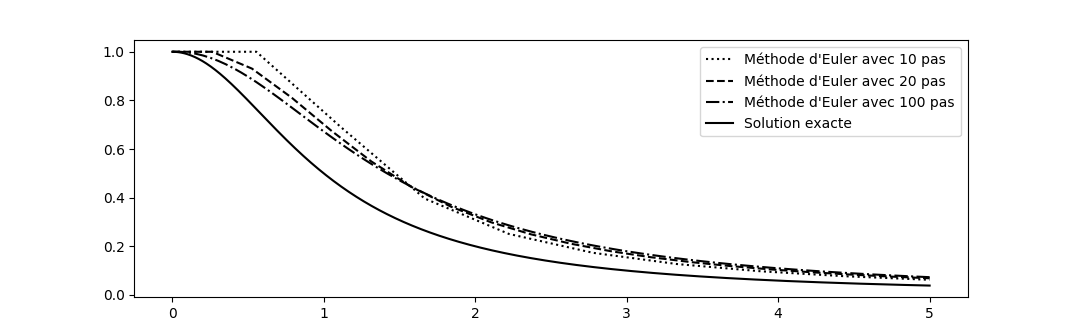
\includegraphics[width=\linewidth]{B-euler}
\end{center}
%--------------------------------------------------------------------------
\subsection{Méthode d'Euler implicite}
%--------------------------------------------------------------------------
Si on approche la fonction à intégrer, $\varphi\bigl(f(u),u\bigr)$, par sa valeur finale sur l'intervalle $[t_k;t_{k+1}]$ c'est-à-dire $\varphi\bigl(u,f(u)\bigr) \simeq \varphi\bigl(f(t_{k+1},t_{k+1})\bigr)\simeq \varphi(y_{k+1},t_{k+1})$ on obtient

\[y_{k+1} =  y_k+\int_{t_{k}}^{t_{k+1}}\varphi(y_{k+1},t_{k+1}) \d u  = y_k+ (t_{k+1}-t_k) \varphi(y_{k+1},t_{k+1})\]
On voit que $y_{k+1}$ apparaît dans le second membre : on ne peut pas le calculer directement.

Pour déterminer $t_{k+1}$ en fonction de $t_k$ il faut donc résoudre, à chaque étape, l'équation $g_k(y)=0$ avec $g_k(y)= y-y_k - (t_{k+1}-t_k) \varphi(y,t_{k+1})$.

On vu que la fonction \type{fsolve} du module \type{scipy.optimize} permet de résoudre cette équation.
%--------------------------------------------------------------------------
\newpage
%--------------------------------------------------------------------------
\subsection{Méthode \type{odeint}}
%--------------------------------------------------------------------------
%--------------------------------------------------------------------------
Le module \type{scipy} contient, dans la sous-bibliothèque \type{integrate} une fonction \type{odeint} qui résout efficacement les équations différentielles. C'est la méthode à utiliser quand la résolution d'une équation est un outil d'un projet plus large.

Ses paramètres sont la fonction qui définit l'équation différentielle, l'ordonnée initiale et un tableau des temps : on doit définir cette liste {\bf avant} d'invoquer la fonction.

Elle renvoie le tableau des valeurs de $y$.
%--------------------------------------------------------------------------
\begin{lstlisting}
import numpy as np
from scipy.integrate import odeint

Y = odeint(f,y0,T)
\end{lstlisting}
%--------------------------------------------------------------------------
%--------------------------------------------------------------------------
\subsection{Méthode de Heun}
%--------------------------------------------------------------------------
%--------------------------------------------------------------------------
La méthode de Heun améliore le schéma d'Euler en approchant l'intégrale par la méthode des trapèzes : $\displaystyle \int_{a}^b g(u) \d u\simeq (b-a)\frac{g(a)+g(b)}2$. On obtient

\[ y(t_{k+1})-y(t_k)\simeq  (t_{k+1}-t_k) \frac {\varphi\bigl(y(t_k),t_k\bigr)+\varphi\bigl(y(t_{k+1}),t_{k+1}\bigr)}2 \]

Cependant cela devient une équation implicite en $y(t_{k+1})$ qu'on ne souhaite pas résoudre.

On va donc procéder en approchant la valeur de $y(t_{k+1})$ dans le second membre par celle que calcule la méthode d'Euler.
\begin{itemize}
\item On calcule $z_k=y_k+\varphi(y_k,t_k)(t_{k+1}-t_k)$ comme valeur approchée de $y(t_{k+1})$
\item On calcule la valeur approchée $\displaystyle y_{k+1} = y_k +
\frac{\varphi(y_k,t_k)+\varphi(z_k,t_{k+1})} 2 (t_{k+1}-t_k)$.
\end{itemize}
%--------------------------------------------------------------------------
%--------------------------------------------------------------------------
\subsection{Méthode de Runge-Kutta}
%--------------------------------------------------------------------------
%--------------------------------------------------------------------------
La méthode de Runge-Kutta s'inspire de la méthode de Simpson : 

\[ \int_{a}^b g(u) \d u\simeq (b-a)\frac{g(a)+4g\bigl(\frac{a+b}2\bigr)+g(b)}6\]

On obtient, pour $m_k = \frac{t_k+t_{k+1}}2$ et $h=t_{k+1}-t_k$,

\[ y(t_{k+1})\simeq y(t_k) + h \frac {\varphi\bigl(y(t_k),t_k\bigr)+4\varphi\bigl(y(m_k),m_k\bigr) + \varphi\bigl(y(t_{k+1}),t_{k+1}\bigr)}6 \]


On va, ici encore, approcher provisoirement les valeurs de $y(m_k)$ et $y(t_{k+1})$.

On va en fait utiliser deux approximations de $y(m_k)$.


\begin{itemize}
\item $a = y_k+\frac{h}2 \varphi\bigl(y_k,t_k\bigr)$ est une première valeur approchée de $y(m_k)$

\item $ b = y_k + \frac{h}2 \varphi\bigl(a, t_k+\frac h2\bigr)$ est aussi une valeur approchée de $y(m_k)$

\item $c = y_k + h \varphi\bigl(b, t_k+\frac h2\bigr)$ est une valeur approchée de $y(t_{k+1})$ obtenue en prenant comme valeur moyenne la valeur au point milieu.
\item On pose alors 

$\displaystyle  y_{k+1} = y_k+ h \frac{\varphi\bigl(y_k,t_k\bigr) + 2\varphi\bigl(a, t_k+\frac h2\bigr) + 2\varphi\bigl(b, t_k+\frac h2\bigr)  + \varphi\bigl(c, t_k+h\bigr)}6$
\end{itemize}
%--------------------------------------------------------------------------
\newpage
%--------------------------------------------------------------------------
\subsection{Cas particulier} 
%--------------------------------------------------------------------------
%--------------------------------------------------------------------------
On voit souvent des équations différentielles d'ordre 2 de la forme $y'' = \psi(y, t)$.

Les conditions initiales forment un couple $(y_0, v_0)$.
%--------------------------------------------------------------------------
\begin{enumerate}
 \item On peut adapter la méthode d'Euler en faisant intervenir une suite des vitesses :
 \[\begin{matrix} y_{i+1} = y_i + (t_{i+1}-t_i)v_i\hfill\\ v_{i+1} = v_i + (t_{i+1}-t_i)\psi(y_i, t_i)\hfill\end{matrix}\]
 Cela revient à résoudre l'équation du premier ordre obtenue par vectorisation.
%--------------------------------------------------------------------------
 \item On peut remarquer qu'on n'a pas besoin de la suite des vitesses si le pas est constant : $t_{i+1}-t_i = \Delta t$ pour tout $i$. 
 \[\begin{matrix} y_1 = y_0 + \Delta t v_0\hfill\\ y_{i+2} = 2y_{i+1} -y_i +(\Delta t)^2\psi(y_i, t_i)\hfill\end{matrix}\]
%--------------------------------------------------------------------------
 \item Si le pas est constant la {\bf méthode de Verlet} améliore la précision en décalant le calcul de l'accélération. On améliore aussi le calcul de $y_1$ car, sinon, on perd le bénéfice de la méthode. 
 \[\begin{matrix} y_1 = y_0 + \Delta t v_0+\frac{(\Delta t)^2}{2}\psi(y_0, t_0) \hfill\\ y_{i+2} = 2y_{i+1} -y_i +(\Delta t)^2\psi(y_{i+1}, t_{i+1})\hfill\end{matrix}\]
%--------------------------------------------------------------------------
 \item Toujours dans le cas d'un pas constant la {\bf méthode saute-mouton} (leapfrog en anglais) donne des résultats précis en entrelaçant dans le temps les calculs de vitesses et de position. On note $w_i$ une approximation de la vitesse au temps $t_i + \frac 12 \Delta t$.
 \[\begin{matrix} w_0 = v_0 + \frac12 \Delta t\psi(t_0,y_0)\hfill\\
 y_{i+1} = y_i + \Delta t w_i\hfill\\ w_{i+1} = w_i + \Delta t \psi(y_{i+1}, t_{i+1})\hfill\\\end{matrix}\]
\end{enumerate}
%--------------------------------------------------------------------------
%--------------------------------------------------------
